\documentclass{amsart}
\usepackage{amsmath}
\usepackage{amssymb}
\usepackage{amsthm}
\usepackage{mathrsfs}
\usepackage{enumerate}
\usepackage{graphicx}
\graphicspath{{../images/}}
\usepackage{courier}
\usepackage{hyperref}
\author{Alex Thies}
\title{Homework 1 \\ Math 463 - Spring 2017}
\begin{document}
	\maketitle

	\noindent{\textbf{Comment}:} I collaborated with Sienna Allen, Joel Bazzle, Torrin Brown, Ashley Ordway, and Seth Temple on this assignment. \\

	\noindent{Here for a vector $\mathbf{y}$ and a subspace $V$, we denote by $\pi(\mathbf{y} | V)$ the projection of $y$ on $V$. Also $\Pi_{V}$ denotes the projection operator onto $V$.}

	\begin{enumerate}
		\item[\textbf{Problem A}] The notation $N(\mu,\sigma^{2})$ means the Normal distribution with mean $\mu$ and variance $\sigma^{2}$.
		Generate values $z_{1},\dots,z_{100},e_{1},\dots,e_{100},d_{1},\dots,d_{100}$ all from a $N(0,1)$ distribution. 
		(Use the R function rnorm. 
		Prior to generating these values, use set.seed with an argument you select, so that your data can be reproduced. 
		Each student must use a different seed value.) 
		Create values, for $i =1,\dots,100$.
			\begin{enumerate}[(1)]
				\item $\mathbf{y}_{i} = 10z_{i}+e_{i}, \ \ \ x_{i} = 8z_{i} + d_{i}$
					\begin{enumerate}[(a)]
						\item Create a scatterplot of $y_{i}$ against $x_{i}$ and superimpose the least-squares line.
						\item Suppose that $x_{50}$ is changed to the value 5. 
						Is the right-hand equation in (1) still true for $i = 50$? 
					\end{enumerate}

					The random vector $(X,Y)$ has a multivariate Normal distribution if there is an $2\times r$ matrix $A$ and a vector $(W_{1},W_{2},\dots,W_{r})$ of independent standard Normal random variables such that that 
						$$\begin{bmatrix}
							X \\
							Y
						\end{bmatrix} 
						= \mathbf{A}\begin{bmatrix}
							W_{1} \\ 
							W_{2} \\ 
							\vdots \\ 
							W_{r} 
						\end{bmatrix}$$
					\item Suppose that $Z$, $\varepsilon$, $\delta$ are i.i.d. each with a standard Normal distribution, and $Y = 10Z + \varepsilon, \ X = 8Z + \delta$. 
					Show that $(X,Y)$ has a multivariate Normal distribution.
					\begin{enumerate}[(a)]
						\item If $(X, Y)$ has a multivariate Normal distribution with $\mu_{X} = \mu_{Y} = 0$, the conditional distribution of $Y$ given $X =x$ is $N(\rho\frac{\sigma_{X}}{\sigma_{Y}}x, (1-\rho^{2})\sigma^{2}_{y})$, where $\rho=\text{corr}(X,Y)$. 
						Find the conditional distribution of $Y$ given $X = x$ for the pair defined in (2).
						\item Find a fixed number $b$ and Normal random variable $\gamma$ so that, for any $x$ the random variable $$Y'_{x} = bx + \gamma$$ has the same distribution as $Y$ given $X = x$.
						\item  Generate $g_{1},\dots,g_{100}$, each with the same distribution as $\gamma$ found above, and set $$y'_{i} = bx_{i} + g_{i}.$$ Plot $\{y'_{i}\}$ against $\{x_{i}\}$. 
						Can you distinguish this plot from the plot made in (a)? 
						What is the least-squares line for this data, and how does it compare to the least-squares line for the data $\{(x_{i}, y_{i})\}$?
						\item What does this exercise say about the ability to infer, based on observational data, the effect of an intervention to change the value of a single variable?
					\end{enumerate}
			\end{enumerate}
		\begin{proof}[Solution]\
			\begin{enumerate}[(1)]
				\item \
				\begin{enumerate}[(a)]
					\item We provide the following plot as instructed, using seed = 38703.
					
					\begin{figure}[h]
						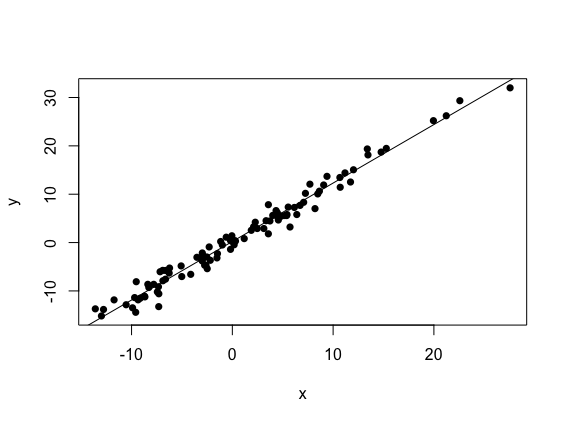
\includegraphics[width=0.6\linewidth]{plot1.png}
						\caption{Scatter plot of random data, with least-squares line}
						\label{fig1}
					\end{figure}

					\item Given that $x$ is a function of the random variables $z$ and $d$ the equation would not hold if we haphazardly changed a value of $x$ without also changing its corresponding inputs.
					I think this follows in a fairly straightforward way from algebra, but I might be thinking about it too simplistically.
				\end{enumerate}

				\item We find that $$\mathbf{A} = 
				\begin{bmatrix} 
				10 & 1 & 0 \\ 
				8 & 0 & 1 
				\end{bmatrix}.$$
				\begin{enumerate}[(a)]
					\item Using the given formulae for the parameters of the conditional distribution for $Y$ given $X = x$ is the following.
					Note that $\sigma_{X} = \sqrt{65}$, $\sigma_{Y} = \sqrt{101}$, $\mathbb{E}(X) = \mathbb{E}(Y) = 0$, and Cov$(X,Y) = 80$.
						\begin{align*}
							\frac{\sigma_{Y}}{\sigma_{X}}\rho x &= \frac{\sqrt{101}}{\sqrt{65}}\cdot \frac{80}{\sqrt{101}\sqrt{65}}, \\
							&= \frac{80}{65}. \\
							&\approx 1.231. \\
							\sigma_{Y}^{2}\left(1 - \rho^{2} \right) &= 101\left(1 - \left( \frac{80}{\sqrt{65}\sqrt{101}} \right)^{2} \right), \\
							&\approx 2.5385.
						\end{align*}
					Hence, the conditional distribution for $Y$ given that $X = x$ is $N(1.231x, 2.5385)$.
					\item Note that $\mathbb{E}(\gamma) = 0$, thus $\mathbb{E}(Y_{x}') = \mathbb{E}(bx) + \mathbb{E}(\gamma) = bx$, thus from previous work we see that $b = 80/65$.
					\item We provide the following plot as instructed,

					\begin{figure}[h]
						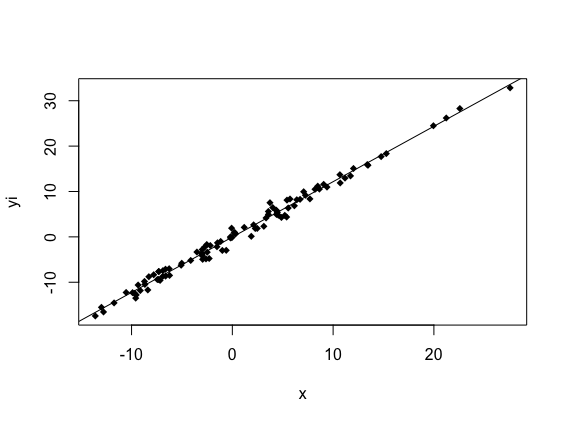
\includegraphics[width=0.6\linewidth]{plot2.png}
						\caption{Scatter plot of slightly altered random data, with least-squares line}
						\label{fig1}
					\end{figure}
					
					While some data points seem shifted slightly, the plots are difficult to tell apart.
					\item The best way that I can describe my thoughts on this, is that changing individual data points does not substantially effect our ability to make predictions with linear models.
				\end{enumerate}
			\end{enumerate}
		\end{proof}
		\newpage

		\item[\textbf{Problem B}] Load the R object gala by \url{load(url("http://pages.uoregon.edu/dlevin/DATA/gala.R"))}
		The variable $\mathbf{y}$ is given in the first column `Species', and the variables $x_{i}$ for $i = 1, 2, 3, 4, 5$ are given by the last four columns. 
		This data records the number of species on islands in the Galapagos chain, along with other geographical and topological variables.
		\begin{enumerate}[(a)]
			\item Find the coefficients $b_{0},b_{1},b_{2},b_{3},b_{4},b_{5}$ of the least-squares fit $$y =b_{0}\mathbf{1}+b_{1}\mathbf{x_{1}} +b_{2}\mathbf{x_{2}} +b_{3}\mathbf{x_{3}} +b_{4}\mathbf{x_{4}} +b_{5}\mathbf{x_{5}} + \mathbf{e}$$ (where $e \perp \mathscr{L}\{\mathbf{1},\mathbf{x_{1}},\dots,\mathbf{x_{5}}\}$) using the function lm in R.
			\item Plot $\mathbf{e}$ against $\mathbf{\hat{y}}$. 
			What does this plot say about the fit of the least-squares linear function?
			\item Compute the least-squares coefficients in R using the matrix multiplication $(\mathbf{X}'\mathbf{X})^{-1}\mathbf{X}'\mathbf{y}$.
			 Note to get a matrix product in R, use \texttt{A\%*\%B}. 
			 The function \texttt{solve} can be used to invert a matrix.
		\end{enumerate}
		\begin{proof}[Solution] \
			\begin{enumerate}[(a)]
				\item We compute $\mathbf{b}$ and $\mathbf{e}$ in R and arrive at the following,
					\begin{align*}
						\mathbf{b} &= \begin{bmatrix}
										7.068221 \\ 
										-0.023938 \\ 
										0.319465 \\ 
										0.009144 \\ 
										-0.240524 \\ 
										-0.074805
									\end{bmatrix}
					\end{align*}
				\item We provide the following plot, as instructed.
					\begin{figure}[h]
						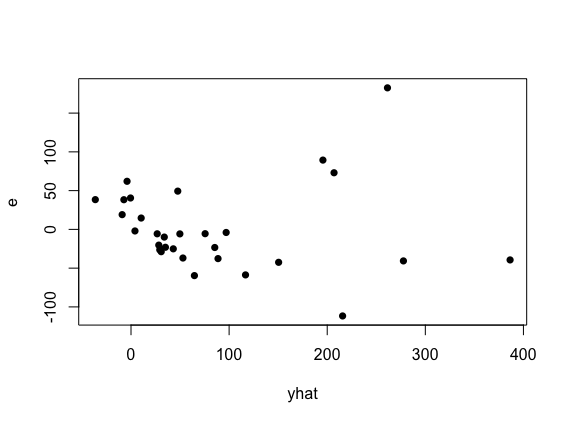
\includegraphics[width=0.6\linewidth]{plot3.png}
						\caption{The slop as a function of the project $\hat{y}$} 
						\label{fig3}
					\end{figure}
				\item We compute the least-squares coefficients in R, as instructed,
					\begin{align*}
						\mathbf{b} &= \begin{bmatrix}
							7.068220709 \\ 
							-0.023938338 \\ 
							0.319464761 \\ 
							0.009143961 \\ 
							-0.240524230 \\ 
							-0.074804832
						\end{bmatrix}
					\end{align*}
			\end{enumerate}
		\end{proof}
		\newpage

		\item[\textbf{Problem C}] Let $\mathbf{y} =(y_{1},\dots,y_{n})'$, $\mathbf{x} =(x_{1},\dots,x_{n})'$, $\mathbf{1}=(1,\dots,1)'$ and $V = \mathscr{L}(\mathbf{1},\mathbf{x})$.
			\begin{enumerate}[(a)]
				\item Use Gram-Schmidt orthogonalization on the vectors $\mathbf{1}$,$\mathbf{x}$ (in this order) to find orthogonal vectors $\mathbf{1}$,$\mathbf{x^{\star}}$ spanning $V$. 
				Express $\mathbf{x^{\star}}$ in terms of $\mathbf{1}$ and $\mathbf{x}$, and find $b_{0}$,$b_{1}$ such that $$\mathbf{\hat{y}} = b_{0}\mathbf{1} + b_{1}\mathbf{x}.$$ To simplify the notation let
				\begin{align*}
					\mathbf{y^{\star}} &= \mathbf{y} - \pi(\mathbf{y}|\mathbf{1}) = \mathbf{y}-\bar{y}\mathbf{1}, \\
					S_{xy} = \langle \mathbf{x^{\star}}, \mathbf{y^{\star}} \rangle = \langle \mathbf{x^{\star}}, \mathbf{y}\rangle = &\sum\limits_{i}(x_{i} - \bar{x})(y_{i} - \bar{y}) = \sum\limits_{i} x_{i}y_{i} - \bar{x}\bar{y}n, \\
					S_{xx} = \langle \mathbf{x^{\star}}, \mathbf{x^{\star}} \rangle = \sum\limits_{i}(x_{i} - \bar{x})^{2} &= \sum\limits_{i} x_{i}^{2} - \bar{x}^{2}n, \\
					S_{yy} = \langle \mathbf{y^{\star}}, \mathbf{y^{\star}} \rangle = \sum\limits_{i}(y_{i} - \bar{y})^{2}&.
				\end{align*}
				\item Suppose $$\mathbf{\hat{y}} = \pi(\mathbf{y}|V) = a_{0}\mathbf{1}+a_{1}\mathbf{x^{\star}}.$$ Find formulae for $a_{1}$ and $a_{0}$ in terms of $\bar{y}$, $S_{xy}$, $S_{xx}$.
				\item  Express $\mathbf{x^{\star}}$ in terms of $\mathbf{1}$ and $\mathbf{x}$, and use this to determine formulas for $b_{1}$ and $b_{0}$ so that $y = b_{0}\mathbf{1} + b_{1}\mathbf{x}^{\star} $.

				\item Express $||\mathbf{\hat{y}}||^{2}$ and $||\mathbf{y} - \mathbf{\hat{y}}||^{2}$ in terms of $S_{xy}$, $S_{xx}$, and $S_{yy}$.
				\item Use the formula $\mathbf{b} = (\mathbf{X}'\mathbf{X})^{-1}\mathbf{X}'\mathbf{Y}$ for $\mathbf{b} = (b_{0}, b_{1})'$ and verify that they are the same as those found in (c).
				\item For $$\mathbf{y} = \begin{bmatrix}
					2 \\
					6 \\
					7 \\
					8
				\end{bmatrix}, \ \ 
				\mathbf{x} = \begin{bmatrix}
					0 \\
					1 \\
					2 \\
					3 
				\end{bmatrix}$$ find $a_{0}$, $a_{1}$, $\mathbf{\hat{y}}$, $b_{0}$, $b_{1}$, $||\mathbf{y}||^{2}$, $||\mathbf{y} - \mathbf{\hat{y}}||^{2}$. Verify that $$||\mathbf{\hat{y}}|| = b_{0}\langle \mathbf{y}, \mathbf{1} \rangle + b_{1} \langle \mathbf{y}, \mathbf{x}\rangle,$$ and that $\mathbf{y} - \mathbf{\hat{y}} \perp V$.
			\end{enumerate}
		\begin{proof}[Solution] \
			\begin{enumerate}[(a)]
				\item We proceed with the Gram-Schmidt orthogonalization algorithm, note that $\mathbf{w}_{1} = \mathbf{1}$.
					\begin{align*}
						\mathbf{w}_{2} &= \mathbf{x} - \frac{\langle x, 1 \rangle}{\langle 1, 1 \rangle}\mathbf{1}, \\
						&= \mathbf{x} - \frac{\sum x_{i}}{n}\mathbf{1}, \\
						&= \mathbf{x} - \bar{x}\mathbf{1}, \\
						&= \mathbf{x}^{\star}.
					\end{align*}
				Observe that $\mathbf{x}^{\star}$ is expressed in terms of $\mathbf{1}$ and $\mathbf{x}$ already. We will skip finding the $b$'s until part (c).
				\item We compute the following,
					\begin{align*}
						\hat{y} &= a_{0}\mathbf{1} + a_{1}\mathbf{x}^{\star}, \\
						&= a_{0}\mathbf{1} + a_{1}x - a_{1}\bar{x}\mathbf{1}, \\
						&= \left(a_{0} - a_{1}\bar{x}\right)\mathbf{1} + a_{1}x.
					\end{align*}
				Thus, we can see that $b_{0} = a_{0} - a_{1}\bar{x}$, $b_{1} = a_{1}$.
				\item We compute the following,
					\begin{align*}
						\hat{y} &= \frac{\langle y, 1 \rangle}{\langle 1,1 \rangle} \mathbf{1} + \frac{\langle y , x^{\star} \rangle}{\langle x^{\star}, x^{\star} \rangle} \mathbf{x}^{\star}, \\
						&= \frac{\sum y_{i}}{n} \mathbf{1} + \frac{yx - y\bar{x}}{S_{xx}}, \\
						&= \bar{y}\mathbf{1} + \frac{S_{xy}}{S_{xx}}\mathbf{x}^{\star}.
					\end{align*}
				Thus, we can see that $a_{0} = \bar{y}$ and $a_{1} = \frac{S_{xy}}{S_{xx}}$
				\item We compute the following,
					\begin{align*}
						||\hat{y}||^{2} &= \langle \hat{y} , \hat{y} \rangle, \\
						&= \langle \bar{y}\mathbf{1}, \bar{y}\mathbf{1}\rangle + 2\left\langle \bar{y}\mathbf{1}, \frac{S_{xy}}{S_{xx}}x^{\star} \right\rangle + \left\langle \frac{S_{xy}}{S_{xx}}x^{\star}, \frac{S_{xy}}{S_{xx}} \right\rangle, \\
						&= \bar{y}^{2}\langle 1,1 \rangle + \left(\frac{S_{xy}}{S_{xy}} \right)^{2}\langle x^{\star},x^{\star} \rangle, \\
						&= n\bar{y}^{2} + \left(\frac{S_{xy}}{S_{xy}} \right)^{2}. \\
						\\
						|| y - \bar{y} ||^{2} &= \langle y - \hat{y}, y-\hat{y}\rangle, \\
						&= \langle y - \bar{y}\mathbf{1} - \frac{S_{xy}}{S_{xx}}x^{\star}, y - \bar{y}\mathbf{1} - \frac{S_{xy}}{S_{xx}}x^{\star} \rangle, \\
						&= \langle y - \hat{y}, y-\hat{y}\rangle + 2\langle y - \bar{y}\mathbf{1}, - \frac{S_{xy}}{S_{xx}}x^{\star} \rangle + \left(\frac{S_{xy}}{S_{xx}}\right)^{2}\langle x^{\star},x^{\star} \rangle, \\
						&= S_{yy} - \left(\frac{S_{xy}}{S_{xx}}\right)^{2}.
					\end{align*}
				\item We compute this in R.
				\item Upon running through the computations I was unable to verify any of what was asked. 
				Given the lack of time remaining to complete the assignment, and my current zombie status due to lack of sleep, I'm calling it good.
			\end{enumerate}
		\end{proof}
		\newpage

		\item[\textbf{Problem D}] Let $\Omega = \mathbb{R}^{4}$, and $$\mathbf{x}_{1} = \begin{bmatrix}
			1 \\
			1 \\
			1 \\
			1
		\end{bmatrix}, \ \ 
		\mathbf{x}_{2} = \begin{bmatrix}
			1 \\
			1 \\
			0 \\
			0
		\end{bmatrix}, \ \ 
		\mathbf{x}_{3} = \begin{bmatrix}
			1 \\
			1 \\
			1 \\
			0
		\end{bmatrix},$$ and let $V_{0} = \mathscr{L}(\mathbf{x}_{4})$ for $\mathbf{x}_{4} =3 \mathbf{x}_{3}-2 \mathbf{x}_{2}$, $V = \mathscr{L}(\mathbf{x}_{1},\mathbf{x}_{2},\mathbf{x}_{3})$. 
		Find $\Pi_{V_{0}}$,$\Pi_{V}$, and $\Pi_{V_{1}}$ for $V_{1}=V_{0}^{\perp}\cap V $. 
		For $\mathbf{y}=(0,2,14,1)'$ find $\pi(\mathbf{y}|V_{0})$, $\pi(\mathbf{y}|V_{1})$, $\pi(\mathbf{y}|V)$.
		\begin{proof}[Solution] We perform the majority of computations here in R, with the script attached.
		First, note that $\mathbf{x}_{1}, \mathbf{x}_{2}, \mathbf{x}_{3}$ are mutually orthogonal, thus we can proceed without the need of Gram-Schmidt orthogonalization of $V = \mathscr{L}(\mathbf{x}_{1}, \mathbf{x}_{2}, \mathbf{x}_{3})$ or $V_{0} = \mathscr{L}(\mathbf{x}_{1}, \mathbf{x}_{2})$.
		We compute the following,
			$$\mathbf{x}_{4} = \begin{bmatrix}
						1 & 1 & 3 & 0
						\end{bmatrix}^{T}.
			$$
			\textbf{Vector Spaces}
			$$V_{0} = \text{span}\begin{bmatrix}
					1 & 1 \\
					1 & 1 \\
					1 & 0 \\
					1 & 0
					\end{bmatrix}, \ \ \ \ 
				V = \text{span}\begin{bmatrix}
					1 & 1 & 1 \\
					1 & 1 & 1 \\
					1 & 0 & 1 \\
					1 & 0 & 0
				\end{bmatrix}
			$$
			\textbf{Projection Operators}
			$$\Pi_{V_{0}} = \begin{bmatrix}
					1/11 & 1/11 & 3/11 & 0 \\
					1/11 & 1/11 & 3/11 & 0 \\
					3/11 & 3/11 & 9/11 & 0 \\
					0 & 0 & 0 & 0
				\end{bmatrix},  \ \ \ \	
			\Pi_{V_{1}} = \begin{bmatrix}
				9/22 & 9/22 & -3/11 & 0 \\
				9/22 & 9/22 & -3/11 & 0 \\
				-3/11 & -3/11 & 2/11 & 0 \\
				0 & 0 & 0 & 1
			\end{bmatrix},
			$$
			$$
			\Pi_{V} = \begin{bmatrix}
				1/2 & 1/2 & -3/11 & 0 \\
				1/2 & 1/2 & -3/11 & 0 \\
				-3/11 & -3/11 & 2/11 & 0 \\
				0 & 0 & 0 & 0
			\end{bmatrix}.
			$$
			\textbf{Projections}
			$$\pi\left(\mathbf{y}|V_{0}\right) = \begin{bmatrix}
				4 \\ 4 \\ 12 \\ 0
			\end{bmatrix}, \ \ \ \
			\pi\left(\mathbf{y}|V_{1}\right) = \begin{bmatrix}
				-3 \\ -3 \\ 2 \\ 1
			\end{bmatrix}, \ \ \ \
			\pi\left(\mathbf{y}|V\right) = \begin{bmatrix}
				1 \\ 1 \\ 14 \\ 1
			\end{bmatrix}.
			$$
		\end{proof}
	\end{enumerate}
\end{document}